\chapter{Results, evaluation and conclusion}\label{ch:results-evaluation-conclusion}

\section{Results}\label{sec:results}

\subsection{Smart contract}\label{subsec:res-smart-contract}

\begin{figure}[H]
    \centering
    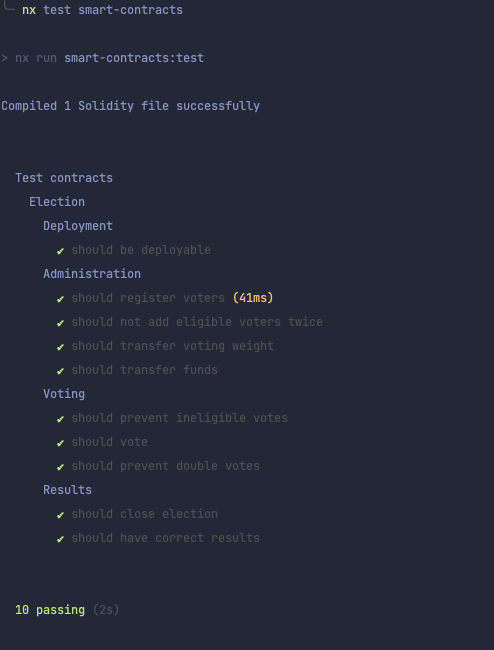
\includegraphics[scale=0.7]{boehm-testing-contract}
    \caption[Smart contract test results]{Smart contract test results. Screenshot taken by author}
    \label{fig:smart-contract-test-results}
\end{figure}

We tested the Solidity code of our \gls{SmartContract} using a JavaScript test suite and the contract's \gls{ABI} (see~\cref{subsec:unit-tests,subsec:testing-the-contract}).
The contract's functions are called in the order they would be called in during an election.
As shown in~\cref{fig:smart-contract-test-results}, the contract's bytecode is deployable to any network that supports Solidity.
Furthermore, all its functions made the expected changes to its internal state and rejected invalid transactions.
Thus, we could show that the contract would ensure a secure election process once deployed (see \cref{subsec:qualitative-objectives,sec:voting-systems}).

\subsection{End-to-end tests}\label{subsec:res-end-to-end-tests}

As seen in~\cref{fig:apx-e2e-tests-1}, we tested the initialization and services of the server's auth module.
In order to prevent users from having multiple accounts, we check entered \glsplural{SSN} and email addresses against our database.
Ultimately, governments would probably implement an \gls{API} in their backend services to validate voters' \glsplural{SSN}.
Regardless of the implementation, our \gls{E2E} tests show that validating a voter's identity by his \gls{SSN} is a secure way for governments to ensure unique accounts, which is one aspect of providing a secure electronic voting system (see \cref{subsec:qualitative-objectives,sec:voting-systems}).

\begin{figure}[H]
    \centering
    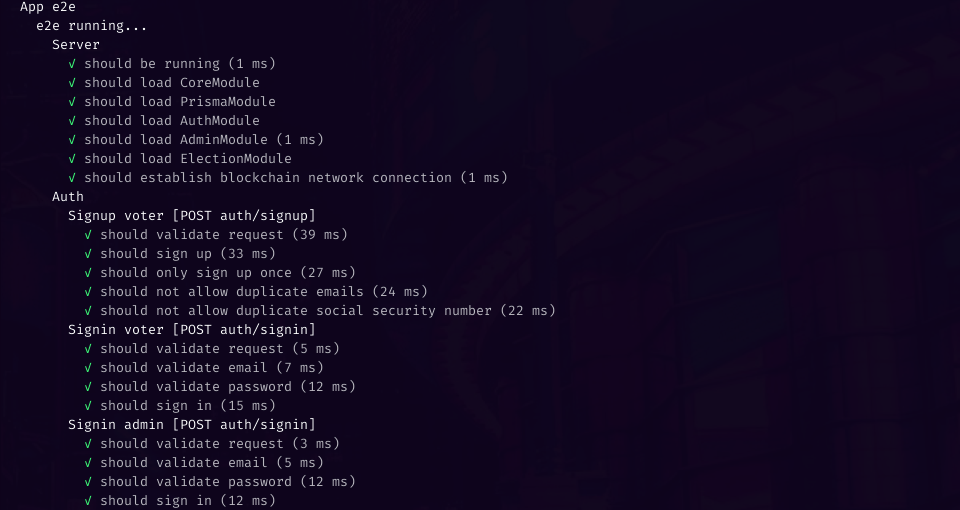
\includegraphics[width=\textwidth-50px]{boehm-e2e-tests1}
    \caption[Server E2E test results of initialization and auth module]{Server E2E test results of initialization and auth module. Screenshot taken by author}
    \label{fig:apx-e2e-tests-1}
\end{figure}

Another aspect is the protection of routes.
Since we aimed to create a system that enables election officials to create and deploy decentralized elections without prior experience developing \glsplural{SmartContract} (see \cref{subsec:quantitative-objectives}), we implemented access control using \glsplural{JWT} (see \cref{subsec:security}).
Consequently, we also tested whether the implemented protection works (see \cref{fig:apx-e2e-tests-2}), showing that \glsplural{JWT} can secure access to server routes.

\begin{figure}[H]
    \centering
    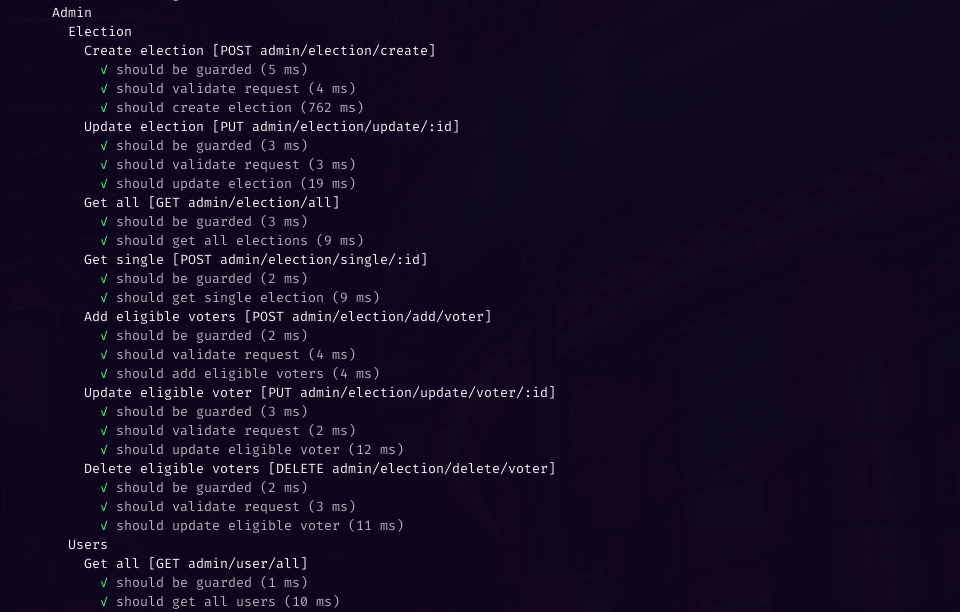
\includegraphics[width=\textwidth-50px]{boehm-e2e-tests2}
    \caption[Server E2E test results of admin module]{Server E2E test results of admin module. Screenshot taken by author}
    \label{fig:apx-e2e-tests-2}
\end{figure}

\begin{figure}[H]
    \centering
    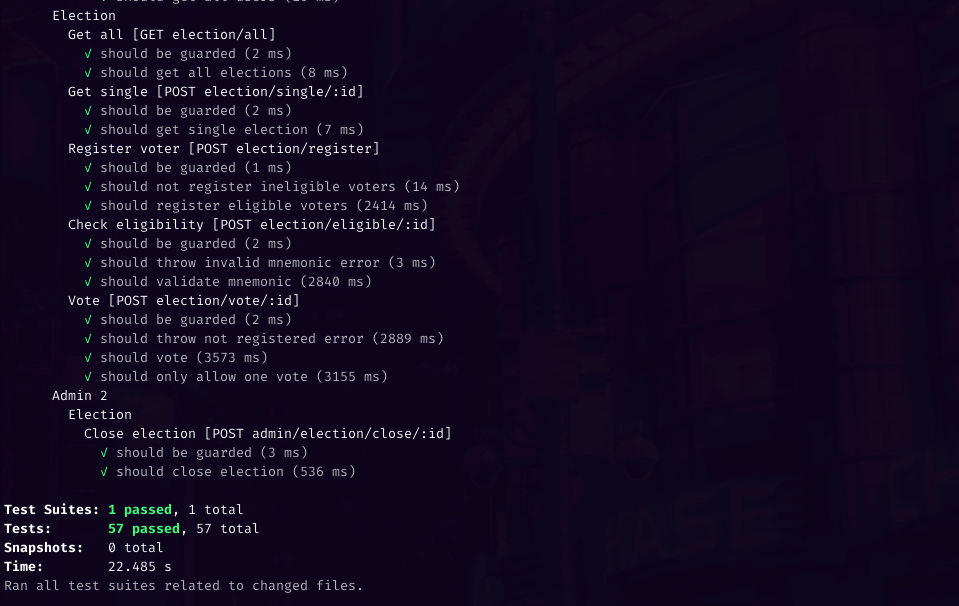
\includegraphics[width=\textwidth-50px]{boehm-e2e-tests3}
    \caption[Server E2E test results of election module]{Server E2E test results of election module. Screenshot taken by author}
    \label{fig:apx-e2e-tests-3}
\end{figure}

The tests were also designed to simulate an \gls{E2E} voting process.
Our \gls{E2E} tests proved that users could not register for an election they are not eligible to vote in (see \cref{fig:apx-e2e-tests-3}).
Also, once they had registered for an election, they could not submit a vote without possessing a registered \gls{PK}-\gls{PBK} key pair since the deployed \gls{SmartContract} only allows transactions from addresses registered in its internal state.
In conclusion, the election's integrity (see \cref{subsec:qualitative-objectives,sec:voting-systems}) is ensured due to the immutability of data stored on \gls{Blockchain} networks (see \cref{sec:blockchain}).

\subsection{Scalability test}\label{subsec:res-scalability-test}

As mentioned in \cref{subsec:quantitative-objectives,sec:voting-systems}, scalability is a crucial feature of any voting system employed in national elections.
In this context, scalability refers to two aspects: processing time, i.e., how much time the system needs to process a number of voters, and the processing cost.
Accordingly, we wrote additional tests that generated high network traffic by simulating a statistically significant number of voters.

\subsubsection{Consecutive votes}\label{subsubsec:res-consecutive-votes}

Simulating consecutive registrations and votes in an election resulted in a processing time of 15000 seconds or 1.5h hours for 1000 voters.
Consequently, it would take 120,000 hours or 164.27 months to process a national election with 80,000,000 eligible voters consecutively.
On the cost side, running the test on Polygon incurred costs of around two MATIC, roughly \$2.00 at the time of this writing.
Moreover, the voting system itself proved to be very reliable when handling consecutive requests, with only five out of 1000 voters being unable to vote, making for a failure rate of .5\%.

\subsubsection{Concurrent votes}\label{subsubsec:res-concurrent-votes}

Unfortunately, the scalability test recorded a 100\% failure rate in concurrent mode.
This could be attributed to a design flaw in our backend services that made the system unable to commit concurrent transactions to the \gls{Blockchain} due to more than one transaction sharing the same transaction nonce.
Consequently, the \gls{Blockchain} network registered those transactions as a single transaction, with the latter trying to modify the first transaction.
We will address this issue in \cref{sec:conclusion}.

\subsection{Transaction analysis}\label{subsec:res-transaction-analysis}

The scalability test generated transactions on the \gls{Blockchain}, enabling us to evaluate voter anonymity, auditability, and scalability regarding transaction costs (see \cref{subsec:qualitative-objectives,sec:voting-systems}).

\subsubsection{Anonymity}

As shown in IMAGE, even though all transactions are publicly visible using a \gls{BlockExplorer}, no identifying information about voters is committed on the \gls{Blockchain} since all transactions are made by our system using a voter's wallet.
Hence, the only information the public will have on an individual voter is his \gls{PBK} and the approximate transaction time.

\subsubsection{Auditability}

The public can independently audit (see \cref{subsec:qualitative-objectives,sec:voting-systems} the election in precisely the same manner, using a \gls{BlockExplorer} to analyze all transactions on the election’s \gls{SmartContract} and to call the contract’s result function to evaluate its internal state of the election result.

\subsubsection{Transaction costs}\label{subsubsec:res-transaction-costs}


\subsection{Quantitative Objectives}\label{subsec:res-quantitaive-objectives}

We aimed to create user interfaces that would take a voter through the \gls{E2E} process of voting in an election while simultaneously providing authorized election officials to create an election without prior experience in \gls{SmartContract} programming (see \cref{subsec:quantitative-objectives}).
As seen in \cref{subsec:pages} appendix video), we achieved all of those objectives.
            The client application of our voting system enables officials to create new elections by filling out a form and registered users to visually identify an election they wish to vote in, register for the selected election and vote for a candidate.

\section{Evaluation}\label{sec:evalutaion}



\section{Conclusion}\label{sec:conclusion}



